\chapter{Progettazione di SPA e utilizzo di framework}


Un framework \'e un'architettura logica di supporto su cui un software pu\'o essere progettato e realizzato al fine di semplificarne lo sviluppo.
Nella progettazione di una spa il suo utilizzo porta notevoli vantaggi, tra cui una migliore organizzazione del codice e l'accesso a funzionalit\'a di livello nettamente superiore rispetto al puro javascript.
Bisogna per\'o tenere conto che il suo utilizzo pu\'o essere visto come una dipendenza, pertanto si avr\'a un prodotto finale pi\'u pesante; star\'a alla sviluppatore decidere se i vantaggi superano i costi.

Ogni framework di JavaScript solitamente incentiva un solo pattern progettuale tra MVC,MVP e MVVM.

%
% Commento: questa � la prima sezione
%
\section{Utilizzo pattern MV*}

\index{?}

%Qui inseriamo un riferimento \cite{a}.

Con il termine mv* si comprende l'insieme dei tradizionali design pattern che utilizzano la suddivisione in model, view e un terzo elemento.
Il model fornisce i metodi per l'accesso ai dati dell'applicazione, mentre il view si occupa della visualizzazione dei dati contenuti nel model e dell'interazione tra utenti e agenti.

Il terzo elemento varia a seconda del pattern utilizzato ed ognuno di essi offre modi diversi per separare i dati dalla logica e dalla rappresentazione dei risultati.
Solitamente i framework si differenziano, oltre che per le eventuali funzionalit\'a diverse, per il tipo di patter mv* che favoriscono durante lo sviluppo dell'applicazione.







\subsection{MVC}
Nel pattern MVC, il primo ideato, il terzo elemento \'e chiamato controller e funge da entry point per l'applicazione.
In questa strategia il controller contiene la logica per elaborare gli input dell'utente e inviare i comandi al model per aggiornare lo stato, il quale si occupa quindi di notificare alla view il cambiamento di stato e quest'ultima accede ai nuovi dati attraverso il model.
\begin{figure}[tp]
    {\begin{center}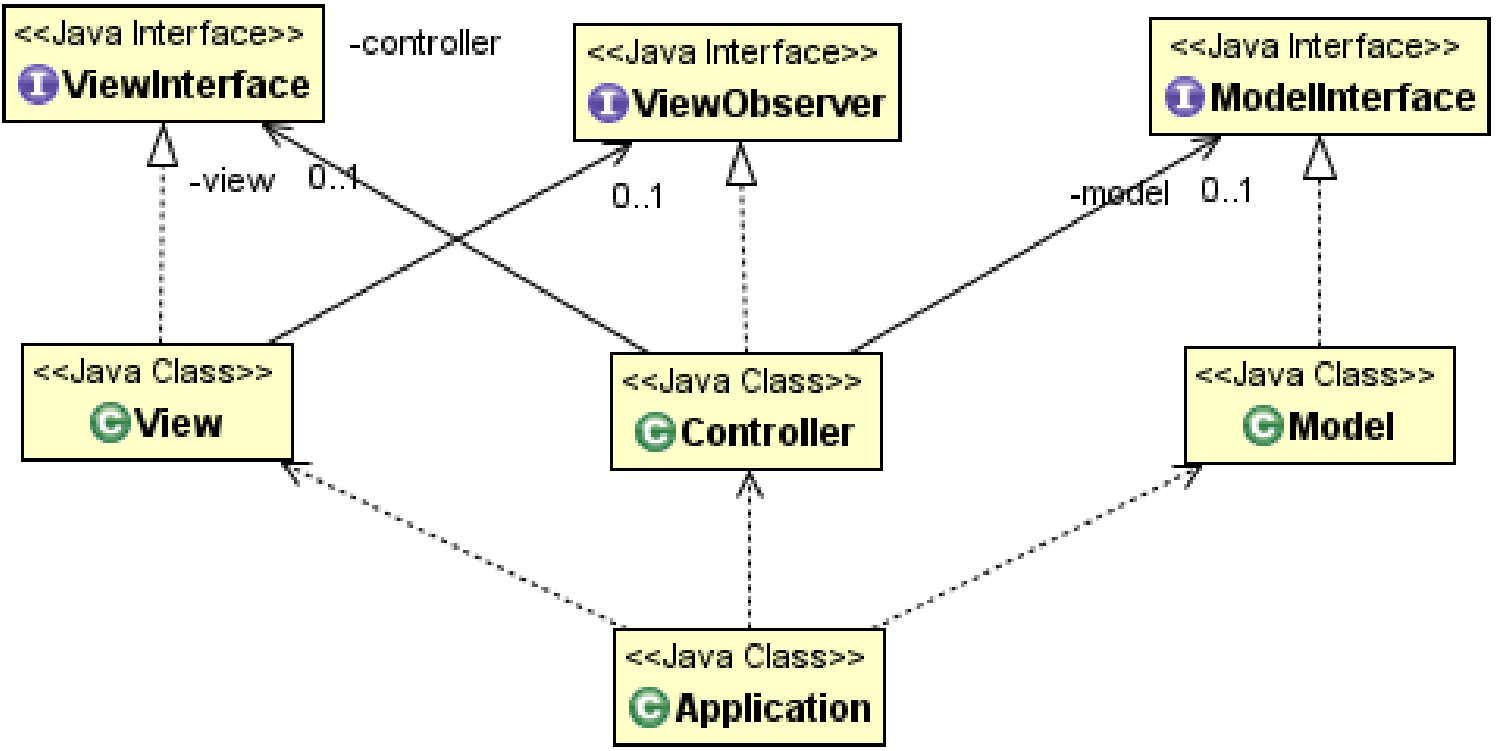
\includegraphics[width=12cm]{figure/mvc.jpg}\end{center}}
\caption{Logica del pattern MVC \label{mvc}}
\end{figure}

La figura ~\ref{mvc} aiuta a comprendere meglio le relazioni tra i vari componenti di questo pattern, in particolare si nota come l'utente interagisca in maniera diretta solo con il Controller e come il model funga da intermediario tra il Controller, la View e i dati.

Questo pattern risulta una buona scelta se la logica, il model e la Unit Interface hanno un livello di complessit\'a tra loro equivalente.
L'uso del MVC risulta efficace nello sviluppo di applicazioni web composte da molte pagine dalle dimensioni contenute, come ad esempio un catalogo.
Il suo utilizzo \'e supportato dal framework Angular.js; \'e presente un esempio dell'utilizzo di questo pattern con Angular.js nella figura ~\ref{mvc_angular}.

In questa figura si pu\'o notare come il model contenga le informazioni del cliente e fornisca, tramite la variabile Cliente, l'accesso al controller dei dati.
La view, passando per il controller, riempie i tag h3 con le informazioni contenute nel model.
\begin{figure}[tp]
{\begin{center}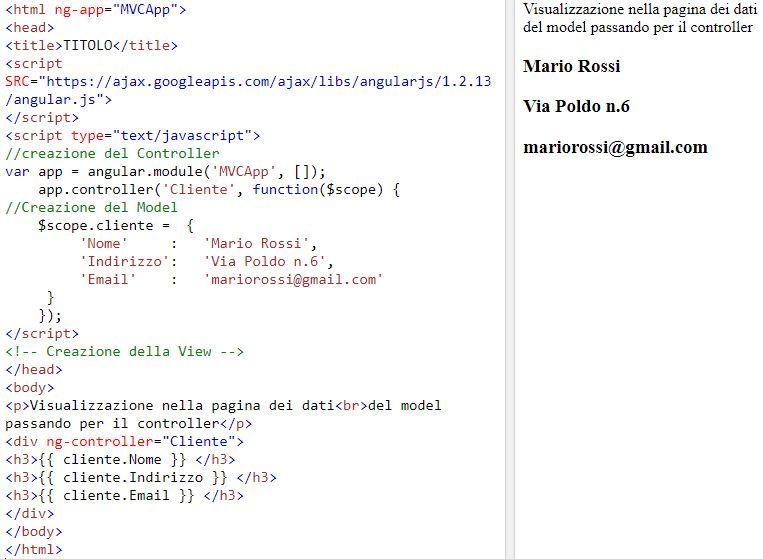
\includegraphics[width=15 cm]{figure/MVC_angular.jpg}\end{center}}
\caption{Utilizzo del pattern MVC con il framework Angular \label{mvc_angular}}
\end{figure}

\subsection{MVP}

Nel pattern MVP, nato come alternativa al pattern MVC, il terzo elemento \'e chiamato presenter e si frappone tra gli altri due componenti.
In questa strategia gli input dell'utente vengono ricevuti dalla view, la quale procede inoltrandoli al presentatore che ha il pieno accesso sul model.
Il model invia delle notifiche al presentatore che si occupa anche dell'aggiornamento della view.

Come si nota nella figura ~\ref{mvp}, questo pattern sposta l'entry point sulla view, concentrandone per\'o la logica nel presentatore che mantiene aggiornati model e view in modo da specializzare i compiti di questi due.
\begin{figure}[tp]
    {\begin{center}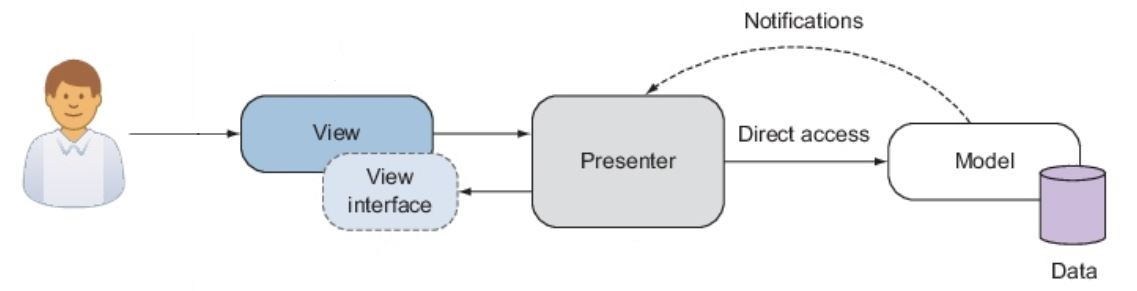
\includegraphics[width=12cm]{figure/mvp.jpg}\end{center}}
\caption{Struttura del pattern mvp  \label{mvp}}
\end{figure}
L'uso del pattern MVP risulta efficace nello sviluppo di applicazioni composte da pagine molto complesse contenenti un elevato numero di funzionalit\'a, come ad esempio un gioco.

\subsection{MVVM}

Il pattern MVVM, sviluppato con l'obbiettivo di semplificare la programmazione ad eventi, vede come terzo componente il model view.
Quest'ultimo svolge una funzione di intermediario tra vista e modello e si occupa della gestione della logica della view; interagisce quindi col modello per ottenere i dati per poi rielaborarli e renderli disponibili in una forma utilizzabile dalla view.\begin{figure}[tp]
    {\begin{center}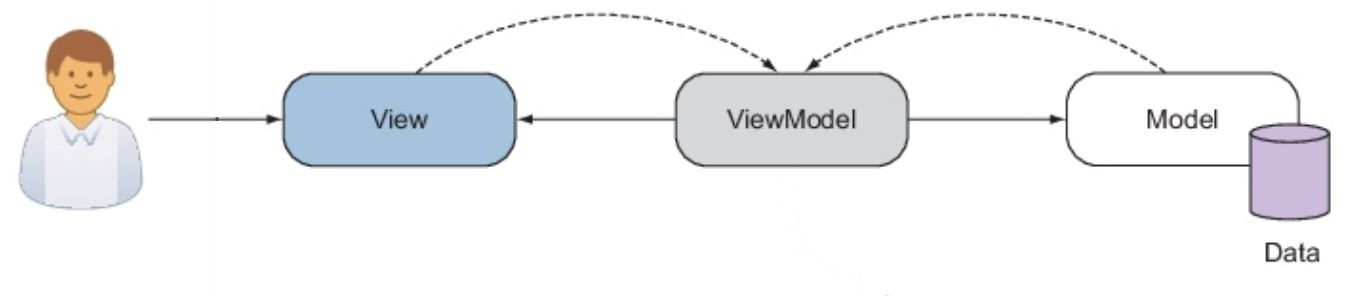
\includegraphics[width=12cm]{figure/mvvm.jpg}\end{center}}
\caption{Struttura del pattern mvvm  \label{mvvm}}
\end{figure}
\section{Modularit\'a}

\index{?}

 Un modulo pu\'o essere definito come una parte  o un componente di qualcosa di pi\'u grande (es: modulo di pagamento) e lo stesso concetto pu\'o essere utilizzato in fase di progettazione di un'applicazione; in particolare nelle spa, le quali hanno spesso un livello di complessit\'a elevato.

JavaScript \'e un linguaggio molto libero e flessibile, di conseguenza si rischia di avere del codice disordinato, per evitare questo problema \'e stato studiato il module pattern che permette una divisione delle varie porzioni di codice in base allo scopo per cui sono state create.

I moduli sono utili non solo per mantenere ordinato il progetto,ma anche per tenere alcune parti di codice private, creare delle API pubbliche richiamabili da altri moduli, evitare conflitti di nomi molto difficili da risolvere in fase di debug e per distinguere facilmente funzioni e variabili con nomi simili.


\subsection{Implementazione}
Non \'e necessario appoggiarsi ai framework per l'implementazione del module pattern, poich\'e pu\'o essere interamente costruito in JavaScript. Per creare un modulo in JS \'e necessario assegnare ad una variabile globale una funzione anonima, dentro la quale si istanzieranno le variabili e le funzioni private; nel return si inseriscono invece le funzioni pubbliche che si vogliono rendere accessibili dal resto del programma.

\begin{figure}[tp]
    {\begin{center}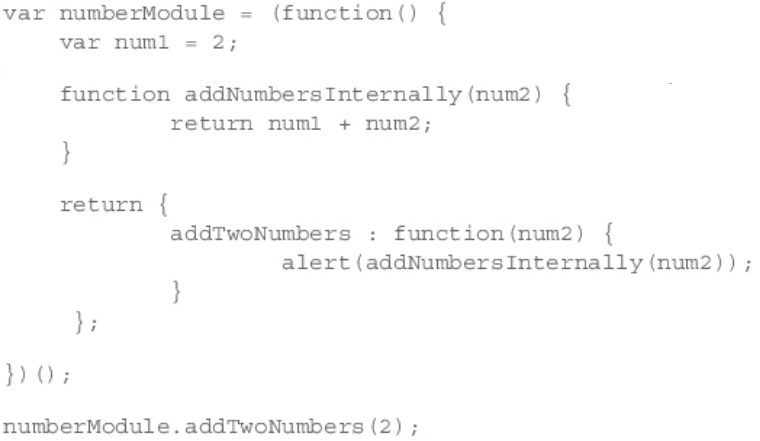
\includegraphics[width=12cm]{figure/codice_modulo.jpg}\end{center}}
\caption{da fare  \label{codice_modulo}}
\end{figure}

Come emerge dall'esempio nella figura ~\ref{codice_modulo}, le funzioni pubbliche possono essere richiamate specificando il nome della variabile globale e la funzione di cui si necessita.
Per applicazioni di piccola grandezza l'uso dei moduli \'e sufficiente a garantire ordine, in applicazioni medio-grandi invece si necessita spesso di un' ulteriore divisione dei moduli in sotto-moduli, che saranno implementati con la stessa logica; diventano quindi delle funzioni pubbliche del primo modulo composte da funzioni pubbliche e private.

Per accedere ad una funzione di un sotto-modulo si deve perci\'o passare sia dal modulo padre che dal secondo modulo, portando ad un ulteriore livello di divisione delle funzioni in base allo scopo.
Una buona pratica, se si hanno dei moduli di una discreta grandezza, \'e dividerli fisicamente in file separati e inclusi nel file HTML dentro ai tag SCRIPT.

\subsection{Ottimizzazione del download delle dipendenze}

Nella maggior parte dei browser il tag SCRIPT blocca la normale esecuzione dell'applicazione finch\'e il download non termina e il codice non viene interamente eseguito.

Per evitare problematiche HTML5 ha introdotto due attributi del tag SCRIPT che migliorano drasticamente il tempo di caricamento della pagina:defer e async.
\begin{enumerate}
\item -Defer: specifica che il codice contenuto nel file venga eseguito solo al completo caricamento della pagina.
\item -Async: specifica che lo script viene venga eseguito in maniera asincrona con il caricamento della pagina
\end{enumerate}

Suddividendo l'applicazione in moduli e salvandoli su file distinti c'\'e per\'o il rischio che una parte dell'applicazione non sia scaricata in tempo e che il corpo principale provi ad eseguire una funzione pubblica di un modulo non ancora completamente scaricato.
In questa eventualit\'a l'utente riscontra inevitabilmente un malfunzionamento, oppure un blocco parziale o totale dell'applicazione.

Per risolvere tale problema sono state sviluppate librerie che gestiscono il download asincrono dei moduli e che permettono l'inizio dell'esecuzione di un modulo solo dopo che tutte le relative dipendenze sono scaricate e disponibili.
Per poter funzionare hanno bisogno di una piccola configurazione nella quale si devono specificare per ogni modulo tutte le dipendenze necessarie, dopo di che la libreria si occuper\'a della gestione dei download e della corretta esecuzione dei moduli.

\section{Router}

\index{?}


La caratteristica che contraddistingue una spa da un'applicazione web multipagina \'e appunto il non dipendere da pi\'u pagine ma di concentrare l'applicazione solo su una.
Nessuna applicazione un minimo complessa pu\'o per\'o essere concentrata in una sola vista, perci\'o \'e necessario un elemento che ci permetta di navigare da una view all'altra passandole eventualmente degli stati.
Questo pu\'o essere risolto, anche se con alcune problematiche, cambiando dinamicamente l'intera view, perdendo per\'o l'utilizzo dei comandi indietro e avanti incorporati nel browser.

Per simulare completamente un'applicazione multipagina (dove questi comandi sono naturalmente supportati) sono state ideate delle tecniche di routing all'interno della spa. 
\begin{figure}[tp]
    {\begin{center}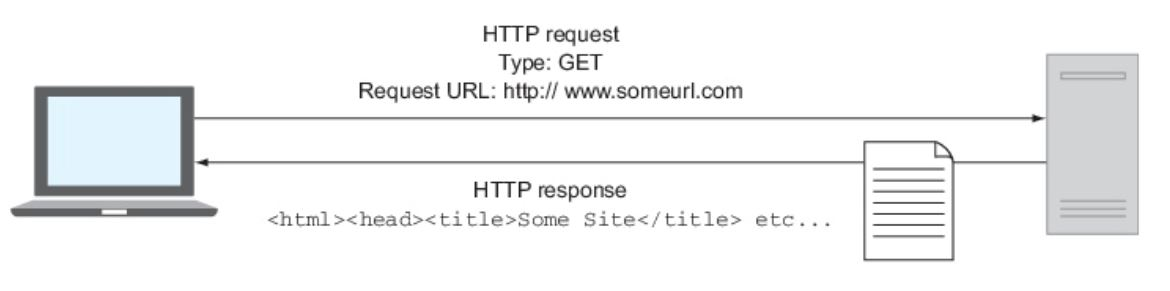
\includegraphics[width=12cm]{figure/no_router.jpg}\end{center}}
\caption{da fare  \label{no_router}}
\end{figure}
\begin{figure}[tp]
    {\begin{center}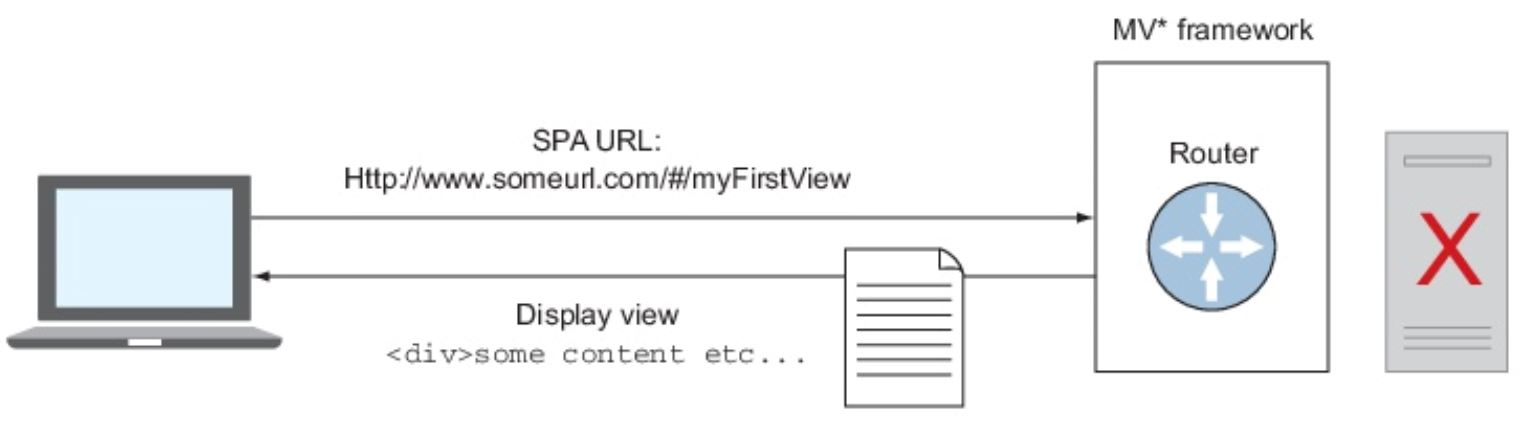
\includegraphics[width=12cm]{figure/si_router.jpg}\end{center}}
\caption{da fare  \label{si_router}}
\end{figure}

Nella figura ~\ref{no_router} \'e possibile osservare il funzionamento di un'applicazione multipagina nella quale, per cambiare la view, \'e necessario effettuare una richiesta al server che ospita la pagina da visualizzare.

Il router invece, come si pu\'o osservare nella figura ~\ref{si_router}, intercetta queste richieste e fornisce istantaneamente le informazioni per visualizzare correttamente la pagina eliminando la necessit\'a di una connessione col server.
 
\subsection{Caratteristiche e funzionalit\'a}

Un ipotetico utente si aspetter\'a di poter utilizzare i normali comandi del browser per muoversi all'interno dell'applicazione e di poter associare ad ogni vista un url univoco.
Per risolvere questo problema sono stati introdotti  all'interno della spa i router che restano in attesa di un evento e, riempendo i <div> del file html, cambiano la view; a questo punto l'utente avr\'a la sensazione che la pagina visalizzata sia completamente nuova.

Alcuni framework possiedono internamente una sorta di router o, in alternativa, \'e possibile includere una libreria esterna specializzata; in entrambi i casi, per\'o, si necessita di una configurazione.

Solitamente, si configurano impostando 4 o 5 campi, a seconda del router:
\begin{enumerate} 
\item name: rappresenta il nome della route.\\*
\item verb: la funzionalit\'a http che si deve intercettare (es. Get).\\*
\item path: il percorso url. Ogni volta che l'url del browser cambia, il router lo compara con questo campo per vedere se combaciano.\\*
\item funzione: questo campo \'e associato a dei comandi che il router deve eseguire quando il path combacia con l'url del browser.\\*
\item view: alcuni router prevedono la possibilit\'a di specificare un file html da caricare come vista.\\
\end{enumerate}

Un cambiamento all'url causa per\'o un refresh della pagina perch\'e il browser, tramite get, cercher\'a di scaricare la risorsa e questo va contro i principi delle spa.
Per evitare questa problematica sono stati ideati due metodi:il primo utilizza il fragment dell'url, mentre il secondo le history API

\subsection{Metodo Fragment Identifier}

Il primo metodo ideato (e il pi\'u compatibile) per evitare il refresh della pagina  prevede l'utilizzo di un fragment identifier univoco per contraddistinguere le varie viste.
Qesto identificatore pu\'o essere una qualsiasi stringa e verr\'a unito all' URL interponendo tra i due il simbolo \#.
Questa seconda parte dell'url viene vista dal browser come un riferimento ad una parte del documento attuale e non ad uno diverso, evitando perci\'o un refresh.


esempio fragment identifier: http://mysite/\#id


Questo identificatore pu\'o essere impostato settando il parametro windows.location.hash = "myId" e aggiunge un nuovo elemento nella cronologia del browser, permettendo quindi all'utente di poter utilizzare i comandi avanti e indietro all'interno della nostra spa.

\subsection{Metodo HTML5 history API}

Il metodo pi\'u recente per evitare il refresh della pagina utilizza invece le API messe a disposizione da html5, in particolare le history API che permettono la manipolazione della cronologia del browser. Tale metodo \'e considerato migliore perch\'e non obbliga lo sviluppatore a creare dei percorsi contenenti obbligatoriamente il simbolo \#.
I due nuovi metodi introdotti da html5 sui quali si basano i router di questo tipo sono i seguenti:
\begin{enumerate} 
\item pushState(): permette l'inserimento di un nuovo indirizzo nella cronologia.\\
\item replaceState(): permette di sovrascrivere un indirizzo nella cronologia con quello attuale.\\
\end{enumerate}
Con il loro utilizzo, il router \'e quindi in grado di modificare l'url visualizzato nel browser senza causare un refresh.
Normalmente, i router all'interno dei framework e delle librerie specializzate supportano entrambi i metodi, sar\'a compito dello sviluppatore scegliere quello pi\'u opportuno per l'applicazione.

\section{AngularJS}

AngularJS \'e un framework scritto in JavaScript con l'obiettivo di risolvere alcuni dei problemi che vengono riscontrati dagli sviluppatori durante lo sviluppo di applicazioni a singola pagina.
Questo framework permette di estendere gli attributi di HTML introducendone alcuni che fungono da direttive; questi poi verranno letti da Angular.js e interpretati.
Tramite questi tag personalizzati lo sviluppatore \'e in grado di legare le parti di ingresso e di uscita della pagina al modello, il quale \'e rappresentato da variabili in JavaScript.
Angular supporta il pattern MVC, ma, grazie alla sua flessibilit\'a, permette anche lo sviluppo di applicazioni con il pattern MVVM e, con pi\'u difficolt\'a, con il pattern MVP; per questo motivo \'e considerato uno dei pochi framework definito MV*.

\subsection {Attributi in AngularJS}

Esistono molti attributi interpretabili da AngularJS ed \'e possibile, per lo sviluppatore, crearne dei nuovi personalizzandone il comportamento.
L'elenco completo delle direttive con le relative descrizioni \'e disponibile presso il sito www.w3schools.com nella sezione dedicata ad Angular.
\begin{figure}[tp]
    {\begin{center}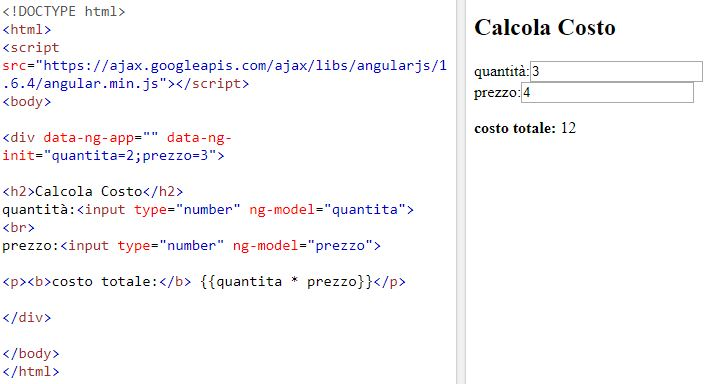
\includegraphics[width=12cm]{figure/angular_es1.jpg}\end{center}}
\caption{Il codice rappresenta una semplice pagina scritta utilizzando AngularJS \label{angular_es1}}
\end{figure}

Nella figura ~\ref{angular_es1} si pu\'o notare che, per poter utilizzare AngularJS, \'e necessario inserirlo tra le dipendenze all'inizio della pagina.
In questo esempio viene creata una semplice applicazione che calcola dinamicamente il costo in base a quantit\'a e prezzo, settabili dall'utilizzatore.
Per ottenere l'aggiornamento dinamico del costo \'e stato utilizzato il tag ng-model per legare i valori degli input alle variabili quantit\'a e prezzo, per poi visualizzarne il prodotto.
Queste variabili sono state inizializzate tramite l'attributo data-ng-init, ma, come si nota nell'esempio, \'e possibile cambiare il valore di queste inserendo un valore negli input; il costo si aggiorna automaticamente al variare del valore di una delle due variabili.

\subsection {Moduli in AngularJS}

La creazione di un modulo pu\'o essere effettuata intermente in JavaScript, spesso per\'o i framework mettono a disposizione dei metodi che semplificano la sua creazione e la gestione delle sue dipendenze.

Angular offre il metodo module(), il quale accetta come parametri una stringa che rappresenta il nome del modulo e un vettore nel quale specificare le eventuali dipendenze.
\'E possibile accedere ad un modulo precedentemente creato passando come singolo parametro la stringa del nome del modulo al quale vogliamo accedere.

La figura ~\ref{mvc_angular} contiene un esempio di utilizzo del metodo module() in AngularJS; nella prima riga viene specificato il modulo(MVCApp) a cui si fa riferimento nella porzione di codice delimitata dai tag html, perci\'o l'oggetto cliente dal quale vengono lette le informazioni \'e contenuto nel controller chiamato Cliente definito nel modulo MVCApp.    

\subsection {Router in Angular.JS}

Angular \'e un framework che supporta l'implementazione dei router per cambiare dinamicamente la view, al fine di facilitare la creazione di un'applicazione a pagina singola.

\begin{figure}[tp]
    {\begin{center}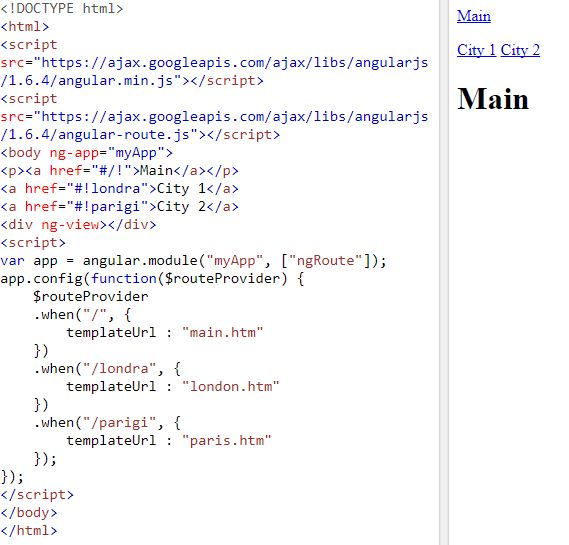
\includegraphics[width=12cm]{figure/angular_router1.jpg}\end{center}}
\caption{Il codice rappresenta una semplice spa implementata in Angular con l'utilizzo dei router \label{angular_router1}}
\end{figure}

Nella figura ~\ref{angular_router1} \'e possibile osservare il codice di una semplice spa che contiene tre pagine, nella quale l'utilizzatore pu\'o muoversi utilizzando i link ad inizio pagina.
Per utilizzare i router \'e necessario, per prima cosa,  aggiungere la relativa dipendenza (angular-route.js), dopo di che \'e possibile utilizzare il modulo ng-Route che si occupa di visualizzare le pagine dell'applicazione senza effettuare operazioni di refresh.
Nella fase di creazione dei link viene specificato il percorso a cui indirizzano il browser nel caso in cui l'utente clicchi su di essi, il router deve essere configurato per intercettare questi percorsi tramite il metodo \$routerProvider.when(), nel quale \'e possibile specificare il percorso da intercettare e il file html da caricare.
\begin{figure}[tp]
    {\begin{center}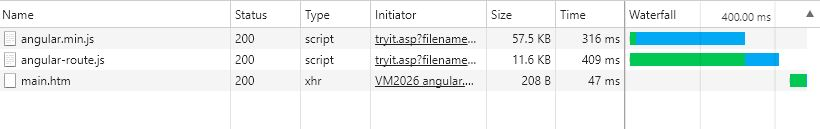
\includegraphics[width=15cm]{figure/angular_router1_download.jpg}\end{center}}
\caption{La tabella rappresenta le risorse di cui l'applicazione nella figura ~\ref{angular_router1} necessita nella fase iniziale\label{angular_router1_download}}
\end{figure}

Nella figura ~\ref{angular_router1_download} si pu\'o notare l'ordine con cui il browser scarica le risorse necessarie all'applicazione nella sua fase iniziale; non sono presenti i file html di londra e parigi perch\'e in questa fase non sono necessari.
\begin{figure}[tp]
    {\begin{center}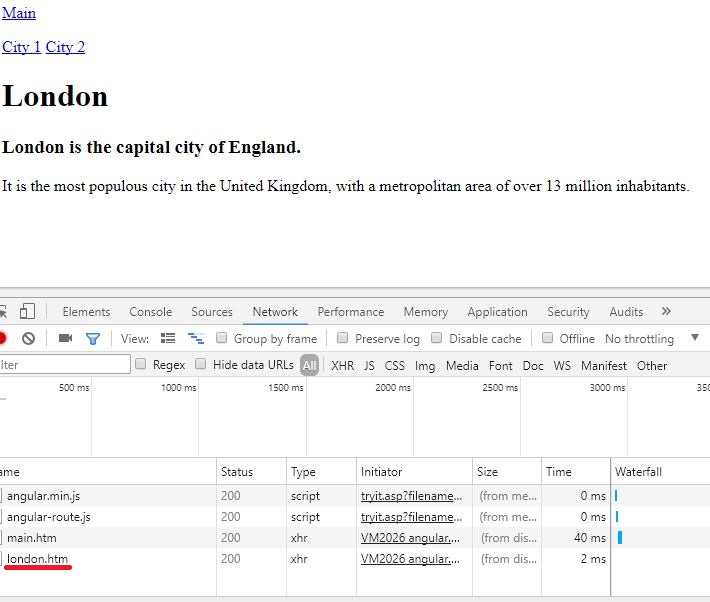
\includegraphics[width=15cm]{figure/angular_router1_londra.jpg}\end{center}}
\caption{Da fare\label{angular_router1_londra}}
\end{figure}

L'immagine ~\ref{angular_router1_londra} dimostra come alla pressione del link da parte dell'utente venga scaricato il file html contenente le informazioni da mostrare, senza causare un refresh di tutta la pagina; tutte queste operazioni sono gestite dal router precedentemente configurato.
Con questa strategia l'utente \'e in grado di muoversi all'interno dell'applicazione anche tramite i tasti indietro e avanti contenuti nel browser, dal momento che vengono aggiunte nella cronologia dal router.
\begin{figure}[tp]
    {\begin{center}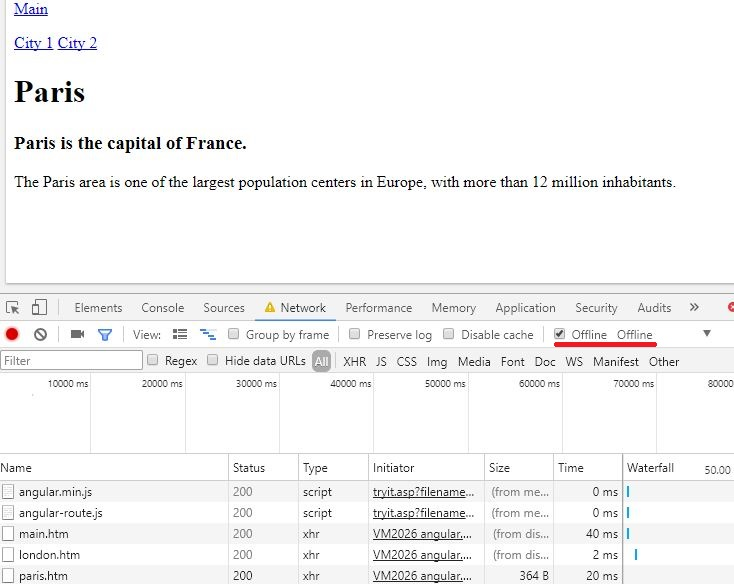
\includegraphics[width=15cm]{figure/angular_router1_parigi.jpg}\end{center}}
\caption{Da fare\label{angular_router1_parigi}}
\end{figure}

Nella figura ~\ref{angular_router1_parigi} sono state scaricate tutte le risorse di cui l'applicazione necessita, a questo punto non \'e pi\'u necessaria alcuna connessione ad internet e l'applicazione \'e in grado di funzionare anche in modalit\'a offline.




